\documentclass[9pt,twocolumn,twoside,lineno]{gsag3jnl}

\articletype{inv} % article type
% {inv} Investigations
% {msr} Mutant Screen Reports
% {gs} Genomic Selection
% {goi} Genetics of Immunity 
% {gos} Genetics of Sex 
% {mp} Multiparental Populations
\usepackage{verbatim}
\usepackage{multirow}

\title{Real Time Genome Scan Using GPU}

\author[$\ast$]{Xiaoqi Hu}
\author[$\ast$]{Hyeonju Kim}
\author[$\ast$]{Saunak Sen}

\affil[$\ast$]{University of Tennessee Health Science Center}

\keywords{Linear Model \\ Genome Scan \\ GPU}

\runningtitle{G3 Journal Template on Overleaf} % For use in the footer 

%% For the footnote.
%% Give the last name of the first author if only one author;
% \runningauthor{FirstAuthorLastname}
%% last names of both authors if there are two authors;
% \runningauthor{FirstAuthorLastname and SecondAuthorLastname}
%% last name of the first author followed by et al, if more than two authors.
\runningauthor{Hu \textit{et al.}}

\begin{abstract}
The BXD strains are an important reference population of
recombinant inbred lines which have been phenotyped extensively.
To facilitate interactive use of genotype-phenotype relationships
in this population, we sought to speed up eQTL scans where we
perform a univariate genome scan for every trait in a collection
of omic traits.  By using easily parallelizable operations such as
matrix multiplication, vectorized operations, and elementwise
operations, we are able to decrease runtimes approaching real-time
computation.  We used parallelization using different CPU threads
as well as GPUs.  We found that the speed advantage of GPUs is
dependent on problem size and shape.  These results indicate a pathway for
speeding up eQTL scans using LMMs.  Our implementation is in the
Julia programming language.

\end{abstract}

\begin{document}

\maketitle
\thispagestyle{firststyle}
\logomark
\articletypemark
\marginmark
\firstpagefootnote

% Use the \equalcontrib command to mark authors with equal
% contributions, using the relevant superscript numbers
\equalcontrib{1}
\equalcontrib{2}

\correspondingauthoraffiliation{3}{Corresponding author: Please insert the affiliation correspondence address and email for the corresponding author. The corresponding author should be marked with the relevant number in the author list, as shown in the example.}
\vspace{-34pt}% Only used for adjusting extra space in the left column of the first page

\noindent        Computational demands in omics are growing exponentially. For
instance, eQTL analysis requires processing genomewide
expression and marker data; this can take minutes, hours or
days depending on problem size.  Scientists want to intereact
with the results and real-time processing would be valuable.
Our goal is to build a backend for GeneNetwork that will enable
real-time genome scans for important genetic reference
populations such as the BXD population.


\section{Methods and Data}
\label{sec:methods:Data}

%Manuscripts submitted to G3 should contain a clear description of the experimental design in sufficient detail so that the experimental analysis could be repeated by another scientist. If the level of detail necessary to explain the protocol goes beyond two paragraphs, give a short description in the main body of the paper and prepare a detailed description for supporting information.  For example, details would include indicating how many individuals were used, and if applicable how individuals or groups were combined for analysis. If working with mutants indicate how many independent mutants were isolated. If working with populations indicate how samples were collected and whether they were random with respect to the target population.

\subsection{Linear Model} 
 Let $y_i$ denote a vector of gene expressions for $n$
individuals in the $i$-th omics trait ( $i=1,\ldots,m$).  We
define a univariate linear model as follows:

\begin{eqnarray*}
	y_i &=& X_j \beta_j+ \epsilon_i,
	\quad \epsilon_i \sim N(0,\sigma_i^2)
\end{eqnarray*}

where ${X}_j$ is a matrix that may include the $y-$intercept with
or without covariate(s), and the $j$-th candidate genetic marker
($j=1,\ldots,p$).  ${\beta}_j$ is a vector of the $j$-th eQTL
effects, and ${\epsilon}_i$ is random error.  Suppose $RSS_{0i}$
is a residual sum of squares under the null hypothesis of no eQTL
and $RSS_{1ij}$ is the residual sum of squares under the
alternative for the $i$-th trait and $j$-th marker.  Then the LOD
score for the corresponding pair can be written as:

\begin{eqnarray*}
	LOD_{ij} &=& \frac{n}{2} \log_{10} \left( \frac{RSS_{0i}}{RSS_{1ij}} \right)\\
	&=& \frac{n}{2} \log_{10} \left( 1{-}r_{ij}^2 \right),
\end{eqnarray*}
where $r_{ij}$ is the correlation between the $i$-th trait and
$j$-th marker. Note that this only works for one-df tests.  If the
trait matrix and genotype matrix ($G$) are standardized, then the
correlation matrix is simply $$R=Y^{'}G.$$
%Indicate which statistical analysis has been performed and describe the method and model applied. If many genes were examined simultaneously, or many phenotypes, a multiple comparison correction should be used to control the type I error rate, or a rationale for not applying a correction must be provided. The type of correction applied should be clearly stated. It should also be clear whether the p-values reported are raw, or after correction. Corrected p-values are often appropriate, but raw p-values should be available in the supporting materials so that others may perform their own corrections. 
Figure \ref{MatrixMult} shows the data layout.
      \begin{figure}[!htb]
	
	\caption{Schematic of data and correlation calculation: $Y$ is
		the expression phenotype matrix, $G$ is the matrix of
		genotytpes, and $R=Y^{\prime}G$ is the matrix of
		correlations.  The LOD scores are a function of the
		correlation matrix.}
	\label{MatrixMult}
	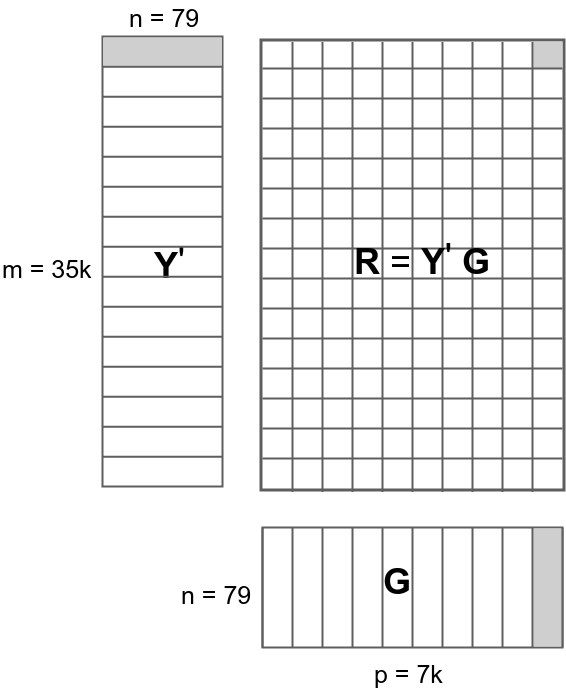
\includegraphics[scale = .4]{figs/YGmatrix.png}
\end{figure}    

\subsection{Acceleration Techniques}
We used various techniques to accelerate eQTL scans. 
\subsubsection{Multithreaded CPU operations}
 Used for multi-threaded loops whenever possible, eg. for element-wise operations
\subsubsection{Matrix and Vectorized Operations}
% OpenBLAS for multi-threaded matrix operations. 
Matrix multiplication is a well studied area where the computer scientists try to apply various optimization techniques to make it run faster. 
There are various BLAS libraries available, such as gslBLAS, OpenBLAS, etc. 
The matrix multiplication in OpenBLAS is default multithreaded, therefore does not require extra coding effort to achieve highly efficient result. 
 
\subsubsection{Single precision}
% Faster and memory efficient; may be less accurate, but acceptable for quick scan
Precision, in computer science, means the smallest difference between two representable numbers.
Floating point numbers, in scientific computing, are usually stored in double presicision. 
Double precision floating point numebrs takes up 8 bytes in memory, while single precision takes up 4 bytes. 
In addition to the difference in storing size, the speed for calculation using single and double precision also varies depending on hardware. 
For example, the GPU throughput (number of floating point calculation per second, measured in FLOPS) for double precision is 1/32 of single precision on a Nvidia GTX 1050 GPU, and 1/4 on a Nvidia Tesla K80. 
Differences in optimization techniques, underlying architecture cause such performance gap. 
Considering the memory size, data transfer speed and throughput, single precision brings multiple benefits when precision is not the priority concern. 


\subsubsection{GPU operations}
\iffalse
% this block is commented out 
	In order to achieve the goal of real time eQTL scans, we profiled the entire process of eQTL scan. Profiling can provide insightful information about the program,  such as running time of each function. 
	Targeting the longest running time functions provides the most gain with limited programming effort and computing resources. 
	In our profiling result, we found that the is calculating correlation matrix and LOD score takes up to 90\% of total running time. 
	Since both steps uses matrix multiplication, which is highly parallelizable and well-researched, we choose the following approaches to speed up matrix multiplication. 
	First, we chose OpenBLAS library for matrix multiplication, which is an optimized  multithreaded BLAS library. 
	In our experiment, gslBLAS (GNU Scientific Library) is 10 times slower than OpenBLAS. 
	In addition to choosing an optimized multithreaded library, we use multithreading operations whenver possible.
	Second, we considered the possibility of using single precision compared to double precision. 
	Precision change will affect both throughput and data transfer time. 
	Throughput is the number of operations done in unit time, usually measured in FLOPS(floating point operations).
	In our experiment, single precision is twice as fast as double precision, and provides correct result within 1e-2 tolerance. 
	Detailed running time of single precision and double precision is show in Table 1. 
	Third, we considered GPU as an attractive computing platform, because of its massive number of cores at a lower price range, and fast open source GPGPU libraries such as CUDA and OpenCL. 
	Matrix multiplication and element-wise operations are amendable to GPU's heterogeneous computing architecture, since both have no data race conditions and low data dependencies. 
	In our experiment, matrix multiplication is up to 5 times faster compared to 16 threaded CPU. 
	We compared the speed of matrix multiplication on CPU and GPU, with rectangular matrix sizes ranging from 1k to 100k, increased by power of 2, 
	We found speed up is sensitive to the size of matrix, and the shape of matrix.  
	GPU is best used for large number of operations, therefore multiplying larger matrices will give better speed up. 
	The shape of matrices also plays an important role when the matrix size is large enough. 
	Figure 2 shows the speed up of matrix multiplication, when the total data size of input and output floating point matrices is over 12 GB. 
	Our reasoning for such sensitivity is that the data transfer from GPU(device) to CPU(host) is half of CPU to GPU. 
	When output data size is larger than input matrix, the speed up will decrease. 
	Further experiment will be done to prove such hypothesis. 
	In addition, our GPU profiling result shows that 98\% of eQTL scan for BXD spleen dataset is spent on data transfer for the GPU approach. 
	Minimizing data transfer time will make the scan significantly faster. 
	Further programming efforts will make GPU a more attractive approach to reach real time eQTL scans. 
	Lastly but most fundamentally, we choose Julia programming language as our development tool. 
	In our experiment of matrix multiplication, Julia's speed is comparable to C/C++. 
	However, the low learning curve, clean syntax, as well as support to GPU programming libraries such as CUDAnative and CuArrays affords much lower programming efforts compared to C/C++.
\fi

%Specialized computations such as matrix multiplications and element-wise operations; requires additional programming effort
Originally used in graphics, GPU has taken off as a general computing device in recent years because of its massive number of cores at a lower price range, and fast GPGPU libraries such as CUDA and OpenCL.
Based on our profiling result, the time consuming parts of our genome scan method are matrix multiplication and element-wise operations. 
Both are amendable to GPU's heterogeneous computing architecture, since they have no data race conditions and low data dependencies. 
However, GPU also has its own limitations. 
To truely utilize the maximum computing power of GPU, one needs to think creatively to work around such limitations from GPU. 
For example, during our experiemnt, memory transfer between host and device is really slow. 
Profiling result shows that 98\% of total genome scan time is spent on memory transfer. 
To cope with this limitation, instead of off-loading the entire correlation matrix, we use GPU to calculate the max lod score of each phenotype, and output the max. 

\subsubsection{Julia language}
%Programming simplicity of interpreted languages with speed approaching compiled languages; GPU programming and linear algebra straightforward
In our experiment of matrix multiplication, Julia's speed is comparable to C/C++. 
However, the low learning curve, clean syntax, as well as support to GPU programming libraries such as CUDAnative and CuArrays affords much lower programming efforts compared to C/C++.
%TODO: Add reference to CUDAnative and CuArrays
\subsubsection{Heritability grid}
For LMMs, considering a discrete grid of heritabilities enhances parallelization


\subsection{Information and Availability of Datasets}
Data from 79 BXD strains for 35556 transcripts from spleens were collected using the Affy Mouse Gene 1.0 ST array. Animals were generated by Drs. Lu, Williams, and colleagues. There were usually one male and one female per strain; strain averages were used as the trait of analysis. All animals were young adults (oldest 160 days). GN accession: GN283. Marker data was available on 7321 markers; genotype probabilities were calculated using R/qtl.

\begin{table*}[htbp]
	\renewcommand{\familydefault}{\sfdefault}\normalfont
	\centering
	\caption{\bf Time comparison between CPU and GPU}
	\begin{tableminipage}{\textwidth}
		\begin{tabularx}{\textwidth}{XXXX}
			\hline
			\header Method & Precision & CPU only   & CPU \& GPU  \\
			\hline
			\multirow{2}{*}{No Find Max LOD} & Single    & 0.36s & 0.41s \\
			& Double    & 0.55s & 0.80s \\
			\multirow{2}{*}{Find Max LOD}    & Single    &1.54s       &0.056s       \\
			& Double    & 1.77s & 0.079s \\
			\hline
			
		\end{tabularx}
		\footnotetext[1]{There are overhead of using GPU, such as data transfer and setting up context, the timing shown for CPU \& GPU here included all overhead for fairness. We ran the genome scan process 10 times and choose the median to remove randomness of each run, and the warm up time of GPU.}
		\label{tab:speedup-table}
	\end{tableminipage}
\end{table*}

 
\section{Results}
\subsection{Benefit of using linear model}
Our method uses linear model, and simplified the genome scan process to basic matrix operations. 
The timing of our method is shown in Table \ref{tab:speedup-table}. 
The execution time without finding the maximum LOD score of phenotype using double precision is 0.55 second if we only use CPU. 
Getting the same result using the same dataset from R/qtl took about 36.5 seconds. 

\subsection{Benefit of using single precision}
Table \ref{tab:speedup-table} also shows the execution time using single and double precisions. 
In all cases, genome scan using single precision runs faster than double precision. 
Using single precision provides benefits in 3 aspects: memory storage, data transfer, and arithmetic calculation. 

\subsection{Benefit of using GPU}
In parallel computing, Amdahl's law is used to find the theoretical maximum speedup by improving a particular part of a program.  
For example, if a program took ten minutes for a serial processor, and a function that takes nine our of those ten minutes can be parallelized, then, the theoretical speedup, no matter how many processors are used, can not be more than ten times, because the minimum execution time of this program is one minute. 
Therefore, profiling the entire genome scan process is the prerequisit in order to begin the optimization. 
Often, profiling would consider space and time complexity. 
Our primary concern is the time taken by each function, therefore only timing information is considered in our profiling. 
We used Julia's built-in Sampling Profiler (%TODO reference here.)
to find our target function for GPU because it is less intrusive compared to other profiling methods. 

The genome scan process includes the following steps:
\begin{itemize}
	\item Calculate standadized matrix for input matrices.
	\item Get correlation matrix
	\item Caclulate LOD score
\end{itemize}
Our profiling result shows that step two and three takes up 90\% of time, and both involve parallelizable matrix operations. 
So they are our candidates for GPU accleration.
To make fair comparison for CPU and GPU, the timing shown in Table \ref{tab:speedup-table} is the total execution time for genome scan. 
The \textit{No Find Max LOD} method shows the timing when running the scan with \textit{CPU only} and \textit{CPU\&GPU}.
As the table shows, the CPU\&GPU combination did not show any improvement over the serial version (CPU only) in terms of time. 
In contrast, it is slower, whether using single or double precision for the data type.
We used a GPU profiler \textit{nvprof} %TODO reference here
to investigate what is the bottleneck of GPU. 
Result is, 98\% of time is spent on data transfer from GPU to CPU (device to host).
As shown in Figure \ref{MatrixMult}, the input matrices Y' and G are small compared to the output matrix R.
For BXD spleen dataset, the Y' and G matrix is about 40MB %TODO: double check on this number
, while R matrix is about 4GB.
For our test hardware Nvidia TESLA V100, data transfer rate from CPU to GPU (host to device) is 4.3GB/s, and GPU to CPU (device to host) is 2.2GB/s. %TODO: double check the numbers here. 
Larger data size at a slower transfer rate makes GPU seems unattractive for computing genome scan, at least for BXD dataset.

To cope with this limitaion of GPU, we further developed \textit{Find Max LOD} method, because main interest of genome scan is to find the maximum LOD score of every phenotype. 
This step is highly parallelizable and can utilize GPU's massive cores, at the same time, reduce the amount of data needed to be transfered back to host. 
Table \ref{tab:speedup-table} shows that \textit{Find Max LOD} method reduces CPU\&GPU execution time down to 0.079 second when using double precision. 
Compared to CPU only, which took 1.77 seconds, this method gains 22 times speedup. 



\begin{figure}[!htb]
	\centering
	\caption{Variation of GPU vs CPU speedup with matrix shape
	}
	\label{GPUCPUShape}
	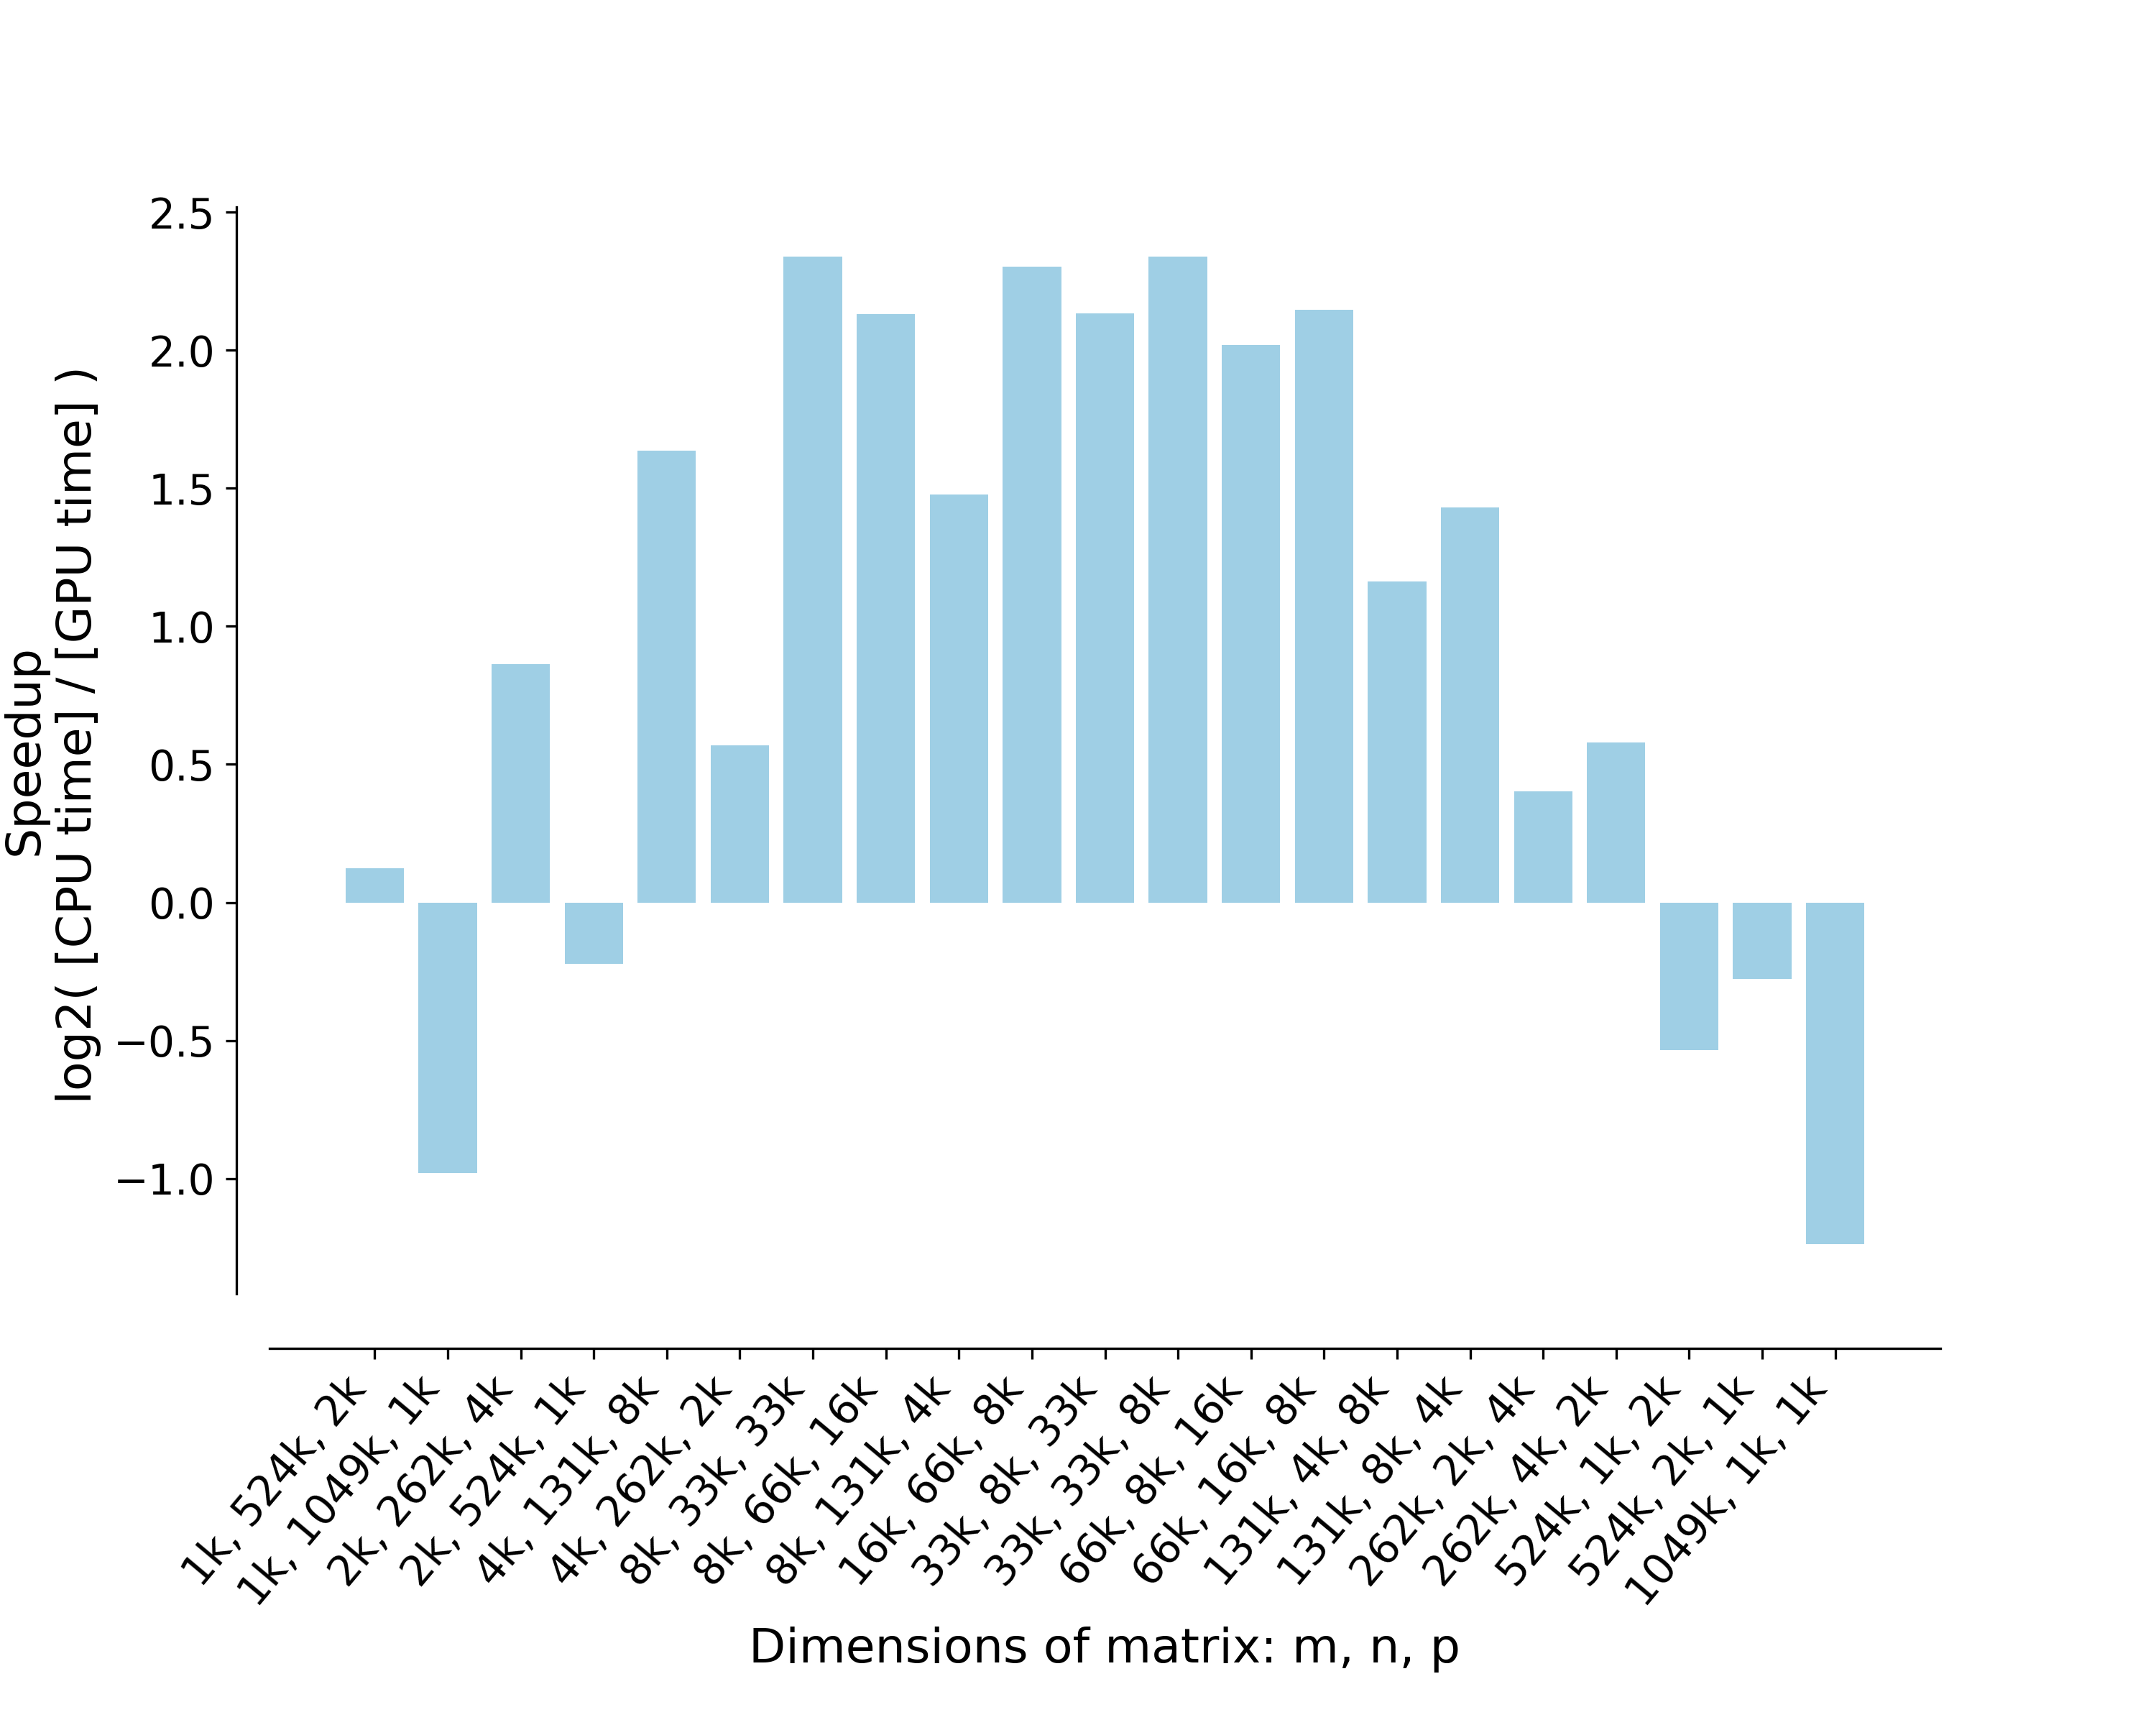
\includegraphics[scale = 0.36]{figs/speedup.png}
\end{figure} 

\iffalse
We profiled the entire genome scan program to get a complete picture of the execution process.
Our profiling result shows that 90\% of runtime is spent on calculating correlation matrix and LOD score. 
Since both involve matrix operations (multiplication and elementwise operations respectively) which are highly parallelizable, we used GPU to speed up matrix operations. 


{\em Profiling:} Calculating correlation matrix and LOD score
takes up to 90\% of runtime.  Both involve matrix operations
(multiplication and elementwise operations respectively) which
are highly parallelizable.
      \begin{itemize}
	\item We chose OpenBLAS library for matrix multiplication, an
	optimized multithreaded library.  In our experiment, gslBLAS
	(GNU Scientific Library) is 10 times slower than OpenBLAS.
	\item We used multithreading operations whenever possible, such as
	for elementwise operations.
	\item We explored using single precision instead of double
	precision.  Precision change affects both throughput (FLOPS) and
	data transfer time.  Single precision is twice
	as fast as double precision, and provides correct result
	within 1e-2 tolerance (Table 1).
\end{itemize}

 {\em GPUs vs CPUs:} GPUs are attractive since they provide a
massive number of cores at a lower price range.
Matrix multiplication and element-wise operations are amendable
to GPU's heterogeneous computing architecture, since both have
no data race conditions and low data dependencies.


\begin{itemize}
	\item Matrix multiplication is up to 5 times faster
	compared to 16-threaded CPU.
	% We compared the speed of matrix
	% multiplication on CPU and GPU, with matrix sizes
	% ranging from 1k to 100k.
	We found speed
	up is sensitive to the size and the shape of matrices.
	% GPU is best used for large number of operations, therefore
	% multiplying larger matrices will give better speed up.  The
	% shape of matrices also plays an important role when the matrix
	% size is large enough.
	Figure 2 shows the speedup of matrix
	multiplication, when the total data size of input and output
	floating point matrices is over 12 GB.
	% Our reasoning for such
	% sensitivity is that the data transfer from GPU(device) to
	% CPU(host) is half of CPU to GPU.
	When output data size is
	larger than input matrix, the speed up will decrease. 
	\item  GPU profiling shows that 98\% of eQTL scan for BXD
	spleen dataset is spent on data transfer.
	Minimizing data transfer time will make the scan significantly
	faster.
\end{itemize}

      {\em Julia as development platform:} In our experiment
of matrix multiplication, Julia's speed is comparable to C/C++.
However, the low learning curve, clean syntax, as well as
support to GPU programming libraries such as CUDAnative and
CuArrays affords much lower programming efforts compared to
C/C++.

\fi


\subsection{Platform}
 \begin{itemize}
	\item CPU: Intel Xeon Gold 6148; 40 cores @ 2.40GHz, 192GB 
	\item GPU: Tesla V100-PCIE; 5120 Cores @ 1380 MHz, 16GB
\end{itemize}
Software: 
\begin{itemize}
	\item Programming environment: Julia; CentOS 7
	\item Libraries: CUDA v10.1 and cuBLAS; OpenBLAS
	\item Profilers: Julia Profiler Package; nvprof
\end{itemize}

%The results and discussion should not be repetitive. The results section should give a factual presentation of the data and all tables and figures should be referenced; the discussion should not summarize the results but provide an interpretation of the results, and should clearly delineate between the findings of the particular study and the possible impact of those findings in a larger context. Authors are encouraged to cite recent work relevant to their interpretations. Present and discuss results only once, not in both the Results and Discussion sections. It is sometimes acceptable to combine results and discussion. The text should be as succinct as possible. Heed Strunk and White's dictum: "Omit needless words!"


\section{Conclusion}


\bibliography{example-bibliography}

\end{document}
